
\documentclass{article}   
\usepackage[utf8]{inputenc}
\usepackage{color}
\usepackage{graphicx} % in the STTT example
\usepackage{amsmath}
\usepackage{amssymb}
\usepackage{mathtools}
\usepackage{algorithm}
\usepackage{multirow}
\usepackage{color}
%\usepackage{amsmath,amssymb,dsfont}
\usepackage{multirow}
\usepackage{algpseudocode}
\usepackage{algorithmicx}
\usepackage{hyperref}
\usepackage{float}
\addtolength{\topmargin}{-100pt}
\addtolength{\textheight}{160pt}

\renewcommand{\textfraction}{0.05}
\renewcommand{\floatpagefraction}{0.90}


\newcommand{\red}[1]{\textcolor{red}{#1}}
\newcommand{\blue}[1]{\textcolor{blue}{#1}}

\newcommand{\IGNORE}[1]{}

\newcommand{\ttit}[1]{{\text{\it #1}}}
\newcommand{\imgchar}[1]{{\bf\small({#1})}}
%\newcommand{\rewrite}{Rewrite}
\newcommand{\Sat}{\text{\it Sat}}
\newcommand{\SatELTL}{\text{Sat{$\exists$}LTL}}
\newcommand{\SatLTL}{\text{SatLTL}}
\newcommand{\SatCTL}{\text{SatCTL}}
\newcommand{\SatCTLstar}{\text{SatCTL*}}
\newcommand{\satCTL}{\Call{satCTL}}
\newcommand{\satLTL}{\Call{satLTL}}
\newcommand{\satELTL}{\Call{sat{$\exists$}LTL}}
\newcommand{\rewrite}{\Call{rewrite}}
\newcommand{\tuple}[1]{{\langle{#1}\rangle}}
\newcommand{\CTLstarMEDD}{{\small RGMEDD*}}
\newcommand{\RGMEDD}{{\small RGMEDD3}}
\newcommand{\ltsmin}{LTSmin}
\newcommand{\greatspn}{GreatSPN}
\newcommand{\meddly}{Meddly}
\newcommand{\spot}{Spot}
\newcommand{\Paths}{\mathbf{\cal P}}
\newcommand{\place}[1]{#1}
\newcommand{\trans}[1]{#1}
\newcommand{\Lang}{\mathcal L}
\newcommand{\AP}{AP}


\newcommand{\PsiRule}{\boldsymbol\Psi}
\newcommand{\phiRule}{\boldsymbol\phi}
\newcommand{\varphiRule}{\boldsymbol\varphi}
\newcommand{\doubleAmp}{\ensuremath{\mathop{\scalebox{0.80}{\&\!\&}}}}
\newcommand{\doublePipe}{\ensuremath{\mathop{\scalebox{0.80}{$||$}}}}

\begin{document}
\title{Esercizio Reti di Petri Produttori e Consumatori}
\author{Lorenzo Dentis}

\date{\today}

\maketitle

\section{Primo setting: 1 produttore, 1 consumatore, 1 buffer a N posizioni}\label{SEC:primo}
\subsection{Primo setting:}
La Petri Net in Figura \ref{FIG:setting1} mostra una basilare rete "producer-consumer" divisibile in 3 sezioni.
\begin{itemize}
	\item Buffer: il buffer ad accesso casuale ad N posizioni è implementato tramite due posti, \emph{buffer} e \emph{buffer\_capacity}.
		Il primo svolge il ruolo di limite minimo, quanti prodotti sono presenti all'interno del buffer; il secondo fa da limite massimo, impedendo che il produttore inserisca più di N elementi.
	\item Producer: Il produttore genera l'elemtento e lo inserisce nel buffer tramite la transizione \emph{place}, tale transizione non è abilitata se non sono presenti token nel posto \emph{buffer\_capacity}, cioè il buffer è pieno
	\item Consumer: Il consumatore preleva un elemento dal buffer (solo se è presente un token nel posto \emph{buffer}) e lo "consuma".
\end{itemize}
Il reachability graph mostra un totale di 8 markings quando $N =1$, il numero di markings aumenta linearmente rispetto al valore $N$.\begin{center}$markings = 4*(N + 1)$\end{center}
\begin{figure*}[!ht]
\centering
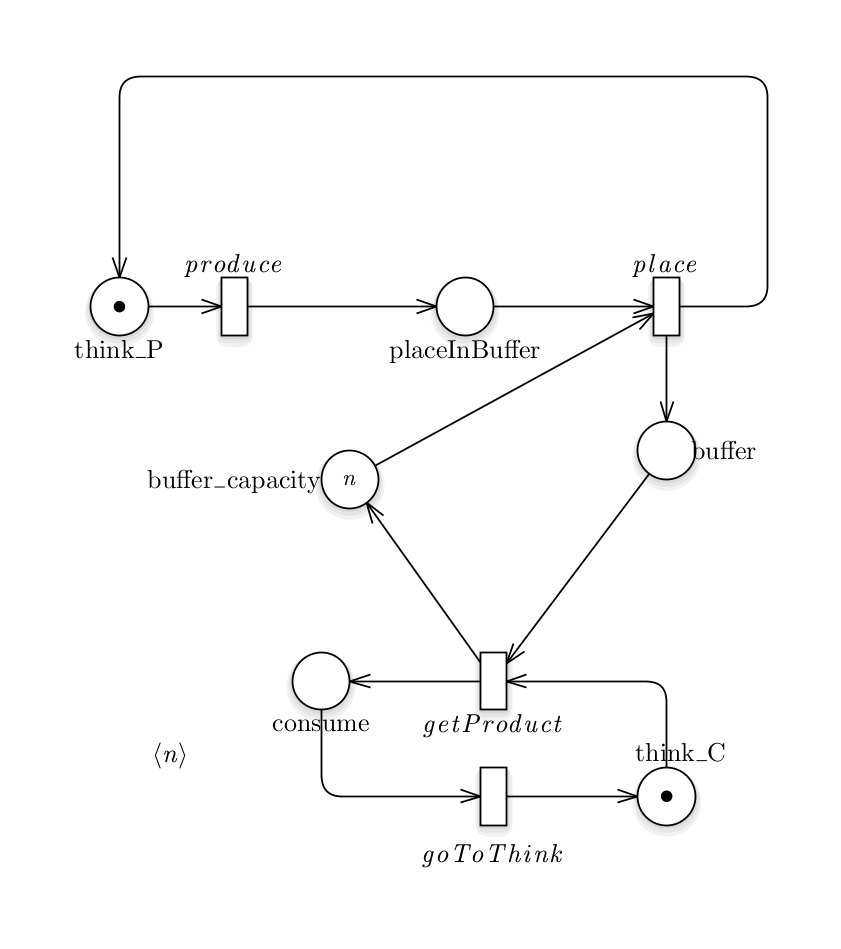
\includegraphics[width=0.6\textwidth]{./Esercizio2_img/setting1.png}
\caption{Setting 1} \label{FIG:setting1}
\end{figure*}
\newpage
\subsection{Rete di petri colorata}
La rappresentazione tramite rete di petri colorata si rivela praticamente identica al caso precendente, a parte la differente notazione le figure~\ref{FIG:setting1} e~\ref{FIG:setting1_CPN} sono identiche.
\begin{figure*}[!ht]
\centering
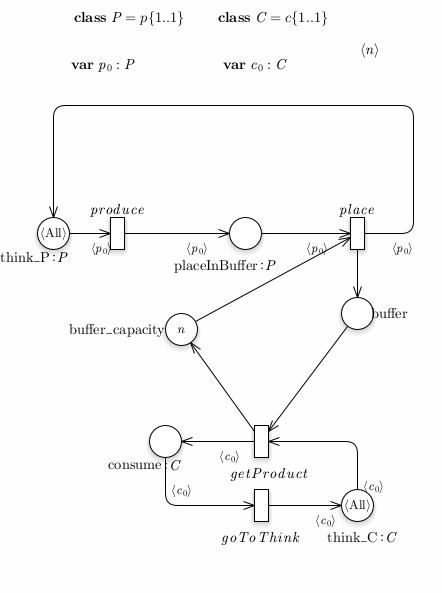
\includegraphics[width=0.8\textwidth]{./Esercizio2_img/setting_1_CPN.png}
\caption{Setting 1 CPN} \label{FIG:setting1_CPN}
\end{figure*}\\
Il reachability graph mostra un totale di 8 markings quando $N =1$, il numero di markings aumenta linearmente rispetto al valore $N$.
Perfettamente in linea con quanto rileato nel caso precendente.
$$markings = 4*(N + 1)$$
Non vi è alcuna differenza tra il RG ed il SRG, essendoci un singolo token nel consumatore ed un singolo token nel produttore non viene generata alcun marking "simbolico".
Una eventuale rete unfolded sarebbe identica a questa rete.
\newpage
\section{Secondo  setting: 1 produttore, 2 consumatori,  1 buffer a N posizioni}\label{SEC:secondo}
\subsection{Secondo  setting: scalatura di marcatura}\label{SEC:secondo-marking}
La soluzione con la scalatura di marcatura richiede di modificare la marcatura del posto \emph{Think\_C}, portando il numero di token a due.\\
L'implementazione è triviale ed il numero di markings mantiene una relazione di linearità rispetto ad $N$.
Per quanto la costante di proporzionalità sia superiore rispetto al caso precedente non vi è un eccessivo incremento di markings anche con valori di $N$ alti.
Ad esempio con $N = 1$ il reachability graph presenta 12 markings mentre con $N = 30$ ne sono presenti 182.\\
La figura \ref{FIG:setting2_markdown} mostra la rete di Petri risultante, praticametente identica alla rete tratta nella sezione precendente (setting \ref{FIG:setting1}). 
$$ markings = 6*(N + 1) $$
\begin{figure*}[!ht]
\centering
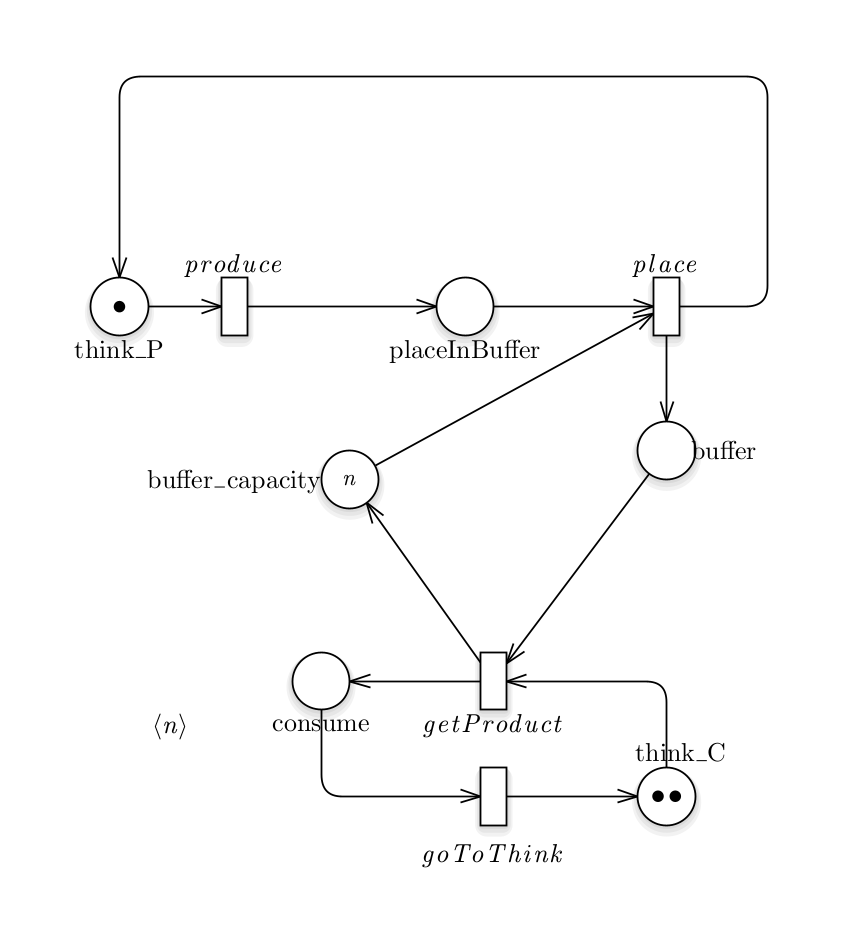
\includegraphics[width=0.75\textwidth]{./Esercizio2_img/setting2_markdown.png}
\caption{Setting 2 con scalatura di marking} \label{FIG:setting2_markdown}
\end{figure*}

\newpage
\subsection{Secondo  setting: replicazione di sottoreti}\label{SEC:secondo-replica}
La soluzione tramite la replicazione della sottorete consumatore presenta una implementazione più complessa e più "scomoda", la rete risultate per quanto meno chiara è ancora di facile comprensione.\\
Il reachability graph è più esteso, con un solo posto nel buffer si ottengono 16 markings e, a differenza dell secondo setting (sezione \ref{SEC:secondo-marking}), la costante di proporzionalità è 8.
Questo porta ad un totale di 248 markings, contro i 182 del caso precedente, quando $N = 30$
$$markings = 8*(N+1)$$.
\begin{figure*}[!ht]
\centering
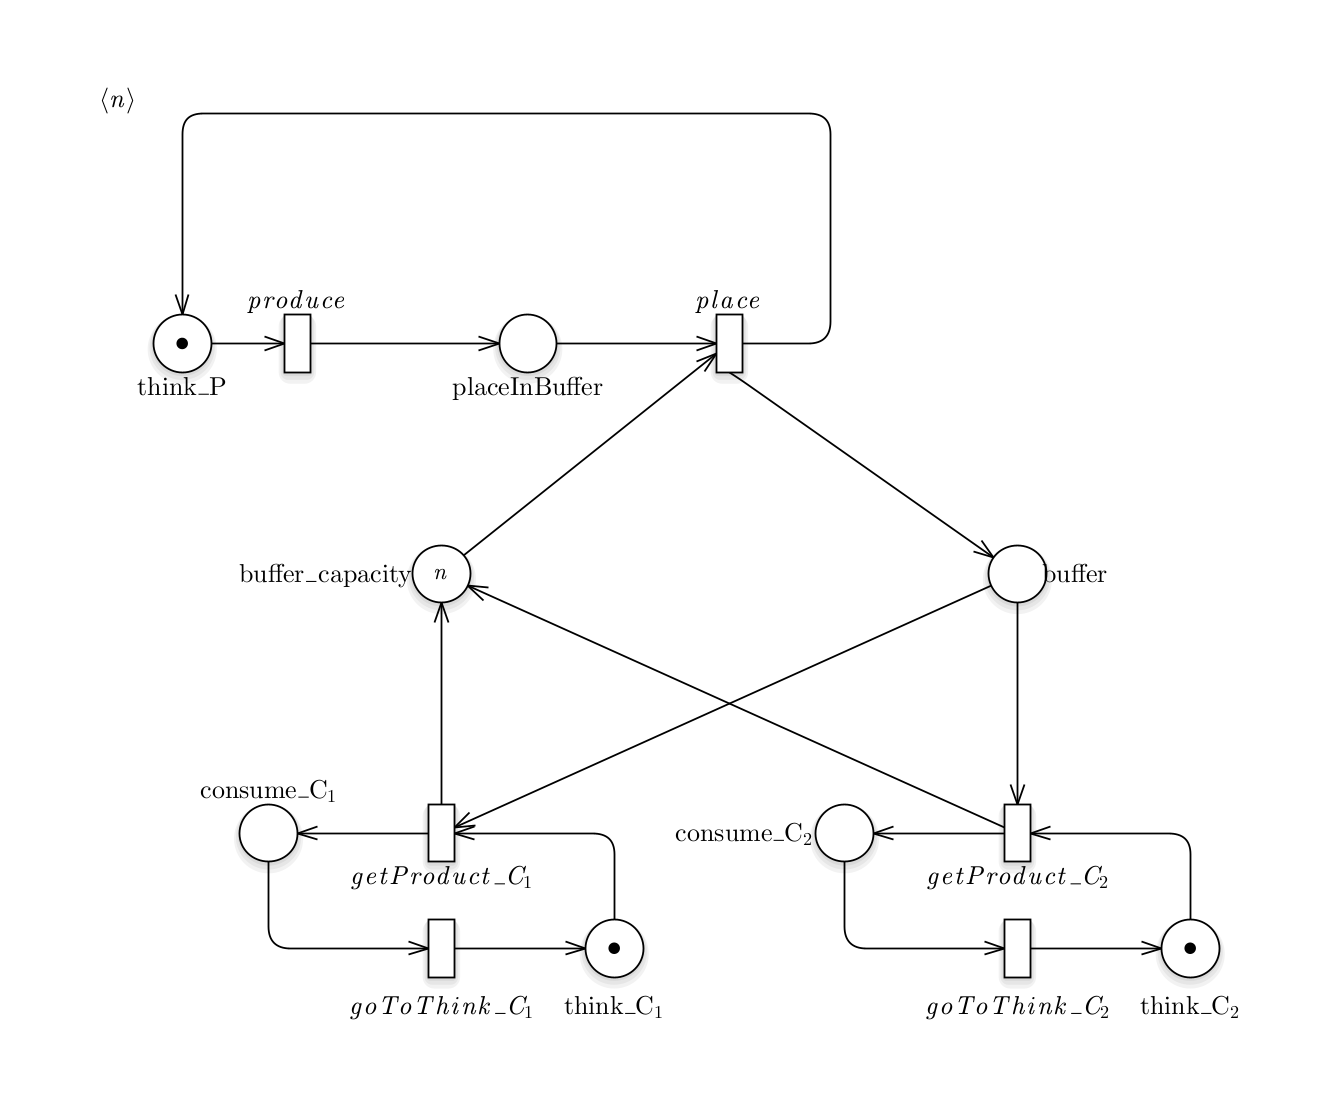
\includegraphics[width=\textwidth]{./Esercizio2_img/setting2_scale.png}
\caption{Setting 2 tramite replicazione} \label{FIG:setting2_scale}
\end{figure*}

\newpage
\subsection{Secondo setting: rete di petri colorata}
Anche questa implementazione si presenta sostanzialmente identica all sezione~\ref{SEC:secondo-marking}.
La marcatura iniziale del posto \textit{Think\_C} viene solamente incrementata di uno e la relazione di linearità del numero di markings del reachability graph rispetto al numero di posti nel buffer viene rispettata.\\
Infatti come ci si aspetterebbe il numero di markings del reachability graph simbolico è identico al numero di marking ottenuto tramite scalatura di marking
\begin{figure*}[!ht]
\centering
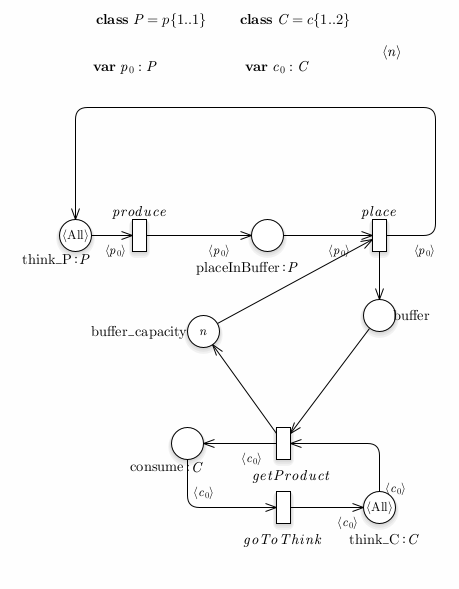
\includegraphics[width=0.75\textwidth]{./Esercizio2_img/setting_2_CPN.png}
\caption{Setting 2 tramite rete di petri colorata} \label{FIG:setting2_CPN}
\end{figure*}
La sostanziale differenza, che è anche il vantaggio che fornisce l'uso delle Reti di Petri colorate, sta nella possibilità di distinguere i due consumatori.\\
I consumatori, che nella sezione~\ref{SEC:secondo-marking} erano indistinguibili, ora sono identificati come $<c_1>$ e $<c_2>$.
Questo senza però dover ricorrere alla scomoda costruzione della sezione~\ref{SEC:secondo-replica}.
La dimensione del Reachability Graph è aumentata di conseguenza,con due soli posti nel buffer sono presenti $24$ markings, con 3 posti $32$ markings e con 4 posti $40$. Esattamente come nel caso~\ref{SEC:secondo-replica}
$$markings = 8 * (N + 1)$$
Questo poichè grazie alla colorazione dei posti è possibile trattare ogni consumatore come se fosse una rete differente, portando il numero di stati del reachability graph allo stesso valore ottenuto separando fisicamente le due reti.
Facendo l'unfolding di questa rete si ottiene la rete ottenuta tramite replicazione di sottoretti.


\newpage
\section{Terzo  setting: P produttori, C consumatori,1 buffer a N posizioni}\label{SEC:terzo}
\subsection{Terzo  setting: scalatura di marcatura}\label{SEC:terzo-marking}
Anche questo setting è di semplice implementazione, come si può vedere in Figura \ref{FIG:setting3_markdown}.Si tratta solamente di inserire dei parametri al posto del marking di Producer e Consumer.
\begin{figure*}[!ht]
\centering
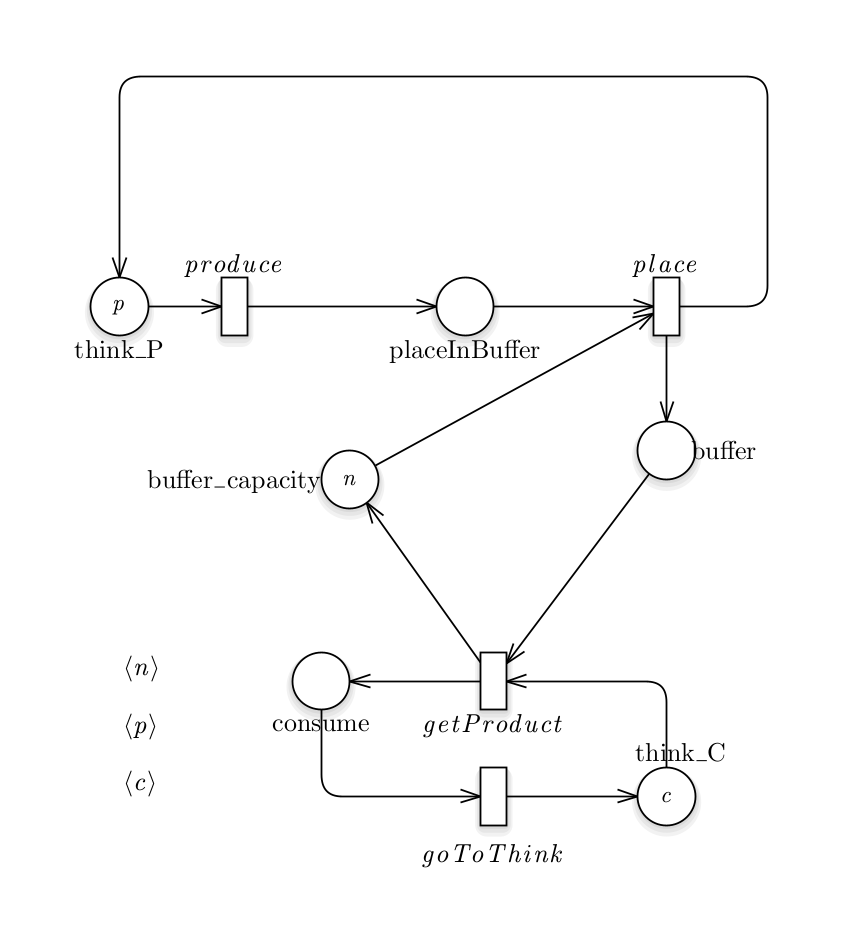
\includegraphics[width=\textwidth]{./Esercizio2_img/setting3_markdown.png}
\caption{Setting 3 tramite la scalatura di marcatura} \label{FIG:setting3_markdown}
\end{figure*}\\
Calcolare come varia esattamente il numero di markings rispetto ai valori $P$, $C$ ed $N$ è complesso, ma al crescere di uno qualsiasi dei parametri l'aumento del numero di markings è comunque limitato, ad esempio impostando un buffer di 4 posti, 4 consumatori e 4 produttori vengono generati 125 markings

%l'equazione corrispondente è\begin{center}$markings = (2N + 2P + (N-1) * (P-1)) * (C+1)$\end{center}
%Ma analizzando l'equazione si può notare che nessuno dei tre parametri ha un influenza maggiore degli altri due.
%Al crescere di $P$, $C$ e $N$ il numero di markings cresce linearmente ed in maniera bilanciata: che sia $P$, $C$ o $N$ ad incrementare non c'è molta differenza nell'incremento dei markings.
\newpage
\subsection{Terzo  setting: replicazione di sottoreti}\label{SEC:terzo-replica}
La metodologia di replicazione delle sottoreti è inadatta a implementare un sistema a $P$ produttori e $C$ consumatori, in quanto se il numero di produttori e consumatori non è noto è impossibile generare manualmente il numero corretto di sottoreti.\\
Una implementazione teorica può essere vista in Figura \ref{FIG:setting3_scale}, ma è appunto solo teorica.
Dato che non ci sono \textbf{realmente} $P$ produttori e $C$ consumatori non si possono usare i tool di analisi di \greatspn.
\begin{figure*}[!ht]
\centering
\centerline{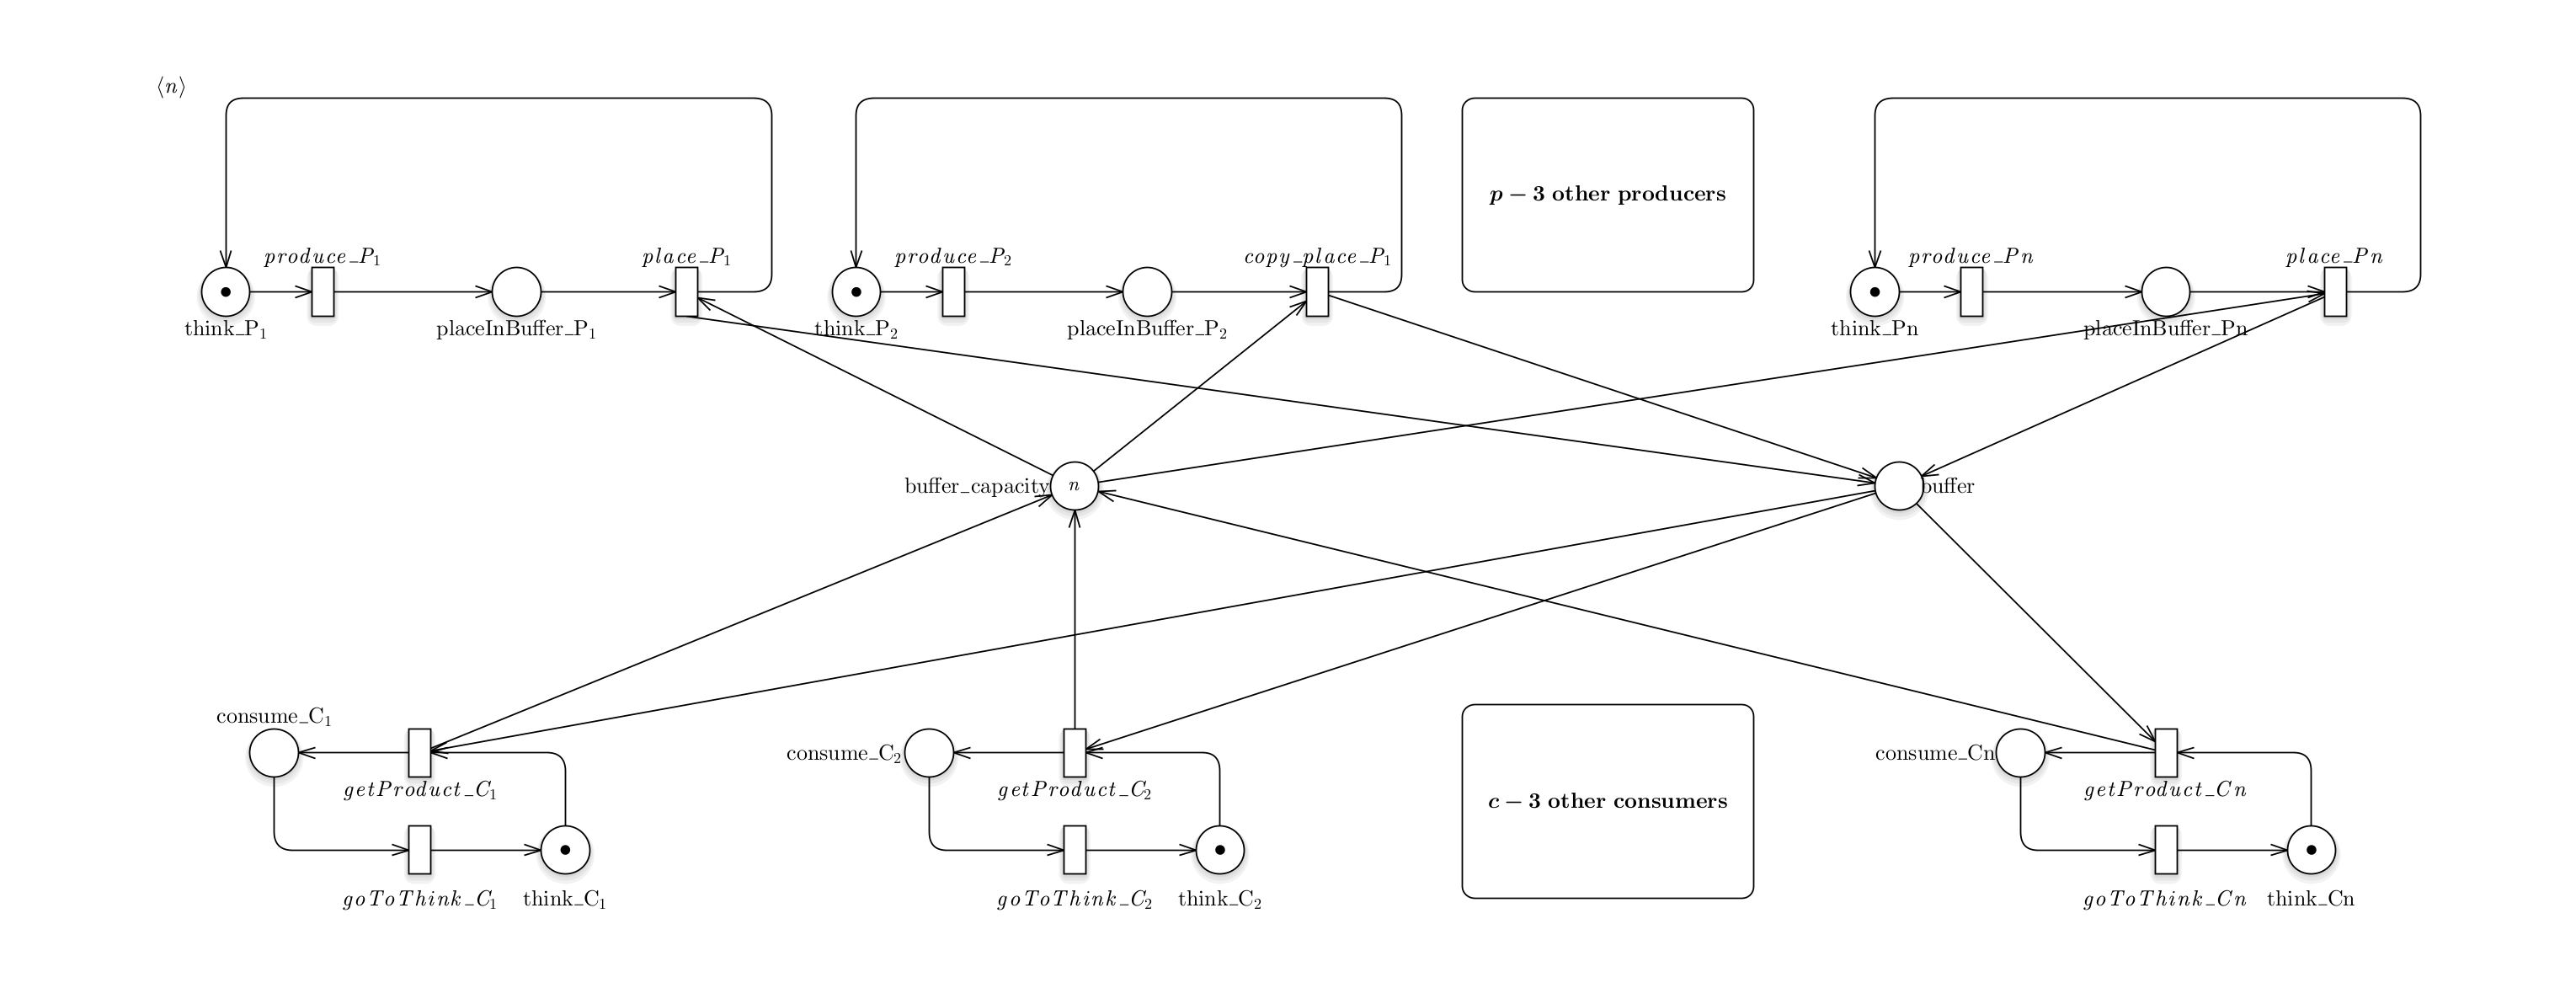
\includegraphics[scale=0.2]{./Esercizio2_img/setting3_scale.png}}
\caption{Setting 3 tramite la scalatura di marcatura} \label{FIG:setting3_scale}
\end{figure*}\\
Comunque volendo fare un'analisi della dimensione del Reachability graph possiamo prendere l'esempio in figura \ref{FIG:setting3_markdown} e confrontarlo con la stessa situazione ma con la scalatura di marcatura, quindi 3 Producer, 3 Consumers e $N$ posti nel buffer.
In questo caso la differenza è notevole, il numero di markings aumenta molto utilizzando il metodo di replicazioni e cresce molto più velocemente, i risultati possono essere osservati in figura \ref{FIG:confronto}.\\
\begin{figure*}[!ht]
\centering
\centerline{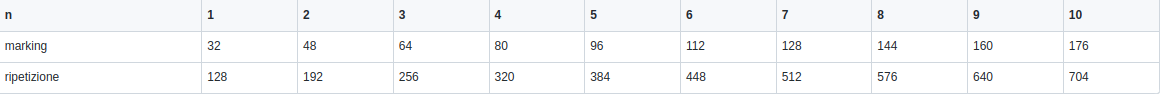
\includegraphics[scale=0.5]{./Esercizio2_img/confronto.png}}
\caption{Setting 3 tramite la scalatura di marcatura} \label{FIG:confronto}
\end{figure*}\\Da questi dati si può concludere che la strategia di replicazione di sottoreti non è vantagggiosa nel dal punto di vista implementativo, ne dal punto di vista della dimensione del reachability graph.
\subsection{Terzo setting: rete di Petri colorata}
Come nel caso precendete (sezione~\ref{SEC:secondo}), l'implentazione tramite rete di Petri colorata combina il vantaggio implementativo della scalatura tramite incremento di marcatura con la distinguibilità della replicazione di sottoreti.\\
Tutti i consumatori sono identificati da un valore $<c_i> \; con \; i \in [1,C]$ ed i produttori dal valore $<p_i> \; con \; i \in [1,P]$ ed è quindi possibile seguirne lo sviluppo e le scelte.
Questo pur mantenendo la raffigurazione chiara e pulita della strategia si scalatura tramite incremento di marking.

Anche in questo caso il numero di marking distinti del reachability graph segue perfettamente il trend della replicazione di sottoreti (vedere figura~\ref{FIG:confronto}).\\
Il \textit{Symbolic Reachability Graph} è identico al \textit{reachability graph} della rete generata tramite scalatura di marking, mentre il \textit{reachability graph} si comporta esattamente come quello che si otterrebbe della rete ottenuta tramite replicazione.\\
Anche in questo caso effettuare unfolding di questa rete colorata porterebbe alla rete della sezione \ref{SEC:terzo-replica}.
\begin{figure*}[!ht]
\centering
\centerline{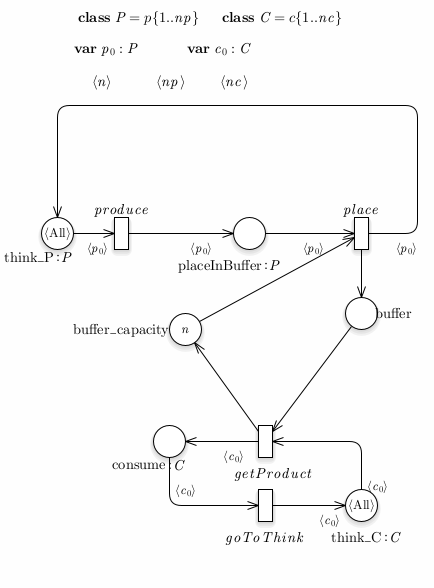
\includegraphics[scale=0.5]{./Esercizio2_img/setting_3_CPN.png}}
\caption{Setting 3 rete di Petri colorata} \label{FIG:setting3_CPN}
\end{figure*}\\

\end{document}
